\chapter{Methodology}
\label{chap:03}
\paragraph{}

Several ideas must be known in order to determine dynamic vibration analysis. There are several elements that impact which model is applied and understood. To determine which model to utilise, the complexity of the system and the number of influencing parameters must be determined. This chapter will go over the different coupled spring mass systems oscillations vibration involving many objects (usually without damping or driving) and how they behave with different parameter values, as well as complex analysis using the Runge Kutta fourth order method (section \ref{RK}) and how to obtain the numerical analysis using software MATLAB. Roughly working, the count of the degree of freedom goes as follows: two and $n^{th}$ for linear systems. To obtain vibration of the two dimensional (2D) spring mass system, which has  one mass and  $n^{th}$ mass respectively. 




\section{Investigate the motion for undamped linear spring mass system with  coupled two degrees of freedom}
\label{2DOF}

The simple one degree of freedom (1DOF) \cite{tsai2020design} systems examined in the preceding section are pretty helpful in developing an understanding of the general properties of vibrating systems. They are far too simplistic to approximate the majority of real-world systems. Real systems have multiple degrees of freedom. Real-world systems are almost never linear. It turns out that they are, but you will not be convinced unless you know how to evaluate more genuine issues and notice how they frequently behave just like the simple idealizations. As early stated in this section spring system of two degrees of freedom (2DOF) \cite{eiss1964vibration} will be discussed with details. 

\subsection{Equations of motion for undamped linear spring mass system with 2DOF }

\paragraph{}
Newton’s second law of motion tells us how a point mass moves in response to a force. But as early stated in this project we use only Lagrange equation (section \ref{lag}) to obtain the equations of motion given coupled systems. In this section, we are given two masses, each of mass $m_1$ and $m_2$, sitting on a frictionless horizontal surface.  The blocks are attached to three springs, and the outer springs are also attached to stationary walls, as shown in figure \ref{fig:7}. The two outer springs each have force constant $k_1$ and $k_3$ respectively, and the inner spring has force constant $k_2$. When the blocks are at rest the springs are unstretched.

Let $_1$ and $x_2$ represent the displacements of mass 1 and 2 from their equilibrium locations, positive to the right. Our goal is to determine the differential equations of motion for each mass and then solve them to determine $x_1(t)$ and $x_2 (t)$. In given figure \ref{fig:6} Degree of freedom (DOF) = 3$\times$2-4 =2 from equation \eqref{1}. Therefore we can say in the figure \ref{fig:6} has two body degree of freedom.



 \begin{figure}[hbt!]
	\centering
	\begin{framed}
	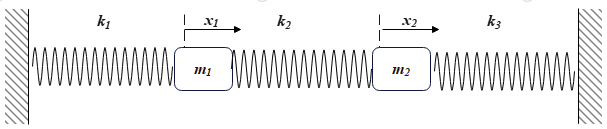
\includegraphics[width=0.7\textwidth]{Figures/G.png}
		\end{framed}
	\caption{ Undamped linear spring mass systems with 2DOF.}
	\label{fig:7}
\end{figure}

In the section, given figure \ref{fig:6} is a two degree of freedom system (2DOF), governed by two differential equations. The governing equations can also be achieved by following Lagrange's Equation directly. The expression for kinetic energy is,

\begin{equation}
    T = \frac{1}{2}m_1\dot{x_1}^2 + \frac{1}{2}m_2\dot{x_2}^2
\end{equation}
And also, the expression for potential energy is,
\begin{equation}
    V = \frac{1}{2}k_1x^2+\frac{1}{2}k_2(x_2-x_1)^2+\frac{1}{2}k_3x_3^2
\end{equation}

 Consider the following seemingly silly combination of the kinetic and potential energies ($T$ and $V$ , respectively), It is denoted by $L$,
\begin{equation}
\label{aaa}
    L = T-V
\end{equation}


Applying Lagrange’s equation to equation \eqref{aaa},
\begin{equation}
    \frac{d}{dt}(\frac{\partial L}{\partial \dot{x1}})-\frac{\partial L}{\partial x1} = 0 
\end{equation}
\begin{equation}
     \frac{d}{dt}(\frac{\partial L}{\partial \dot{x2}})-\frac{\partial L}{\partial x2} = 0
\end{equation}

Governing differential equations \cite{cartwright1945non} are based on balance laws for mass and momentum, and completed by constitutive relations for the fluid and solid phases as well as their mutual interactions. In the section  equation \eqref{aaa} its results we can obtain the governing equations as,

\newpage

\begin{equation}
\label{aab}
    m_1\dot{x_1}+(k_1+k_2)x_1-k_2x_2=0
\end{equation}
\begin{equation}
\label{aac}
    m_2\dot{x_2}-k_2x_1+(k_2+k_3)x_2 = 0
\end{equation}

Clearly,  we were able to realised for multi degree of freedom systems, this approach (Lagrangian) has advantages over the force balancing approach using Newton’s law.

\subsection{Matrix form of equations of motion}

\paragraph{}

To approach vibration problems, we always put the equations of motion (\eqref{aab} and \eqref{aac}) in matrix form. The matrix form of the system of governing equations of motion is as follows and the component matrices are commonly named as listed below. 
\begin{equation}
    M \frac{d\dot{x^2}}{dt}+ Kx = 0
\end{equation}

\begin{equation}
\label{aad}
    [M]{\dot{X}}+[K]{X} = 0
\end{equation}

\begin{gather}
 \begin{bmatrix} m_1 & 0 \\ 0 & m_2 \end{bmatrix} \frac{d^2}{dt^2} \begin{bmatrix}
  x_1 \\ x_2
 \end{bmatrix} + \begin{bmatrix}
  k_1+k_2 & -k_2 \\ -k_2 & k_2+k_3
 \end{bmatrix}
 \begin{bmatrix}
  x_1 \\ x_2
 \end{bmatrix}
 =
  \begin{bmatrix}
0 \\0
   \end{bmatrix}
\end{gather}

\begin{gather}
    \begin{bmatrix}
m_1 & 0\\0& m_2 
\end{bmatrix}{\dot{X}} +
\begin{bmatrix}
k_1+k_2 &-k_2\\-k_2&k_2+k_3
\end{bmatrix}{X} = 0
\end{gather}


Where $x$ is a vector of the variables describing the motion,  $M$ is called the ‘mass matrix’ and $K$ is called the ‘Stiffness matrix’ for the system. $M$ and $K$ are 2$\times$2 matrices for a system with two masses (or, more broadly, two degrees of freedom). They are $n \times n$ matrices for a system with $n$ degrees of freedom.

\subsection{Natural frequencies and mode shapes for 2-degrees-of-freedom undamped linear system}
\paragraph{}

First. now let us go over the definitions of natural frequencies and mode shapes first. Remember that we may make a system vibrate by slightly pushing it from its static equilibrium state and then releasing it. The resulting motion will not be harmonic in general. Certain special initial displacements, on the other hand, will result in harmonic vibrations. These unique initial deflections are known as mode shapes, and the accompanying vibrational frequencies are known as natural frequencies \cite{kuether2014numerical} \cite{gigerenzer2011natural}. A vibrating system's natural frequencies are its most essential attribute. It is useful to have a straightforward method for calculating them.

To continue, we need to make the crucial assumption that the system has specific motions in which both masses oscillate at the same frequency. We will observe that for one-dimensional chains, there seem to be exactly as many normal modes as there are masses in the system. Each and every normal mode corresponds to a single frequency of motion, but the frequencies of normal modes can be vary. We may represent the general motion of any mass in terms of a superposition of normal modes once we have identified the movements associated with the normal modes and determined the normal mode frequencies. Assume that both masses move at the same frequency to find the normal mode frequencies.

\begin{equation}
\label{x1}
    x_1 = A_1e^{i\omega t}
\end{equation}

\begin{equation}
\label{x2}
    x_2 = A_2e^{i\omega t}
\end{equation}

Consider the double derivation of equation \eqref{x1} and \eqref{x2},

\begin{equation}
\label{x1}
    \Ddot{x_1}  = - \omega^2 A_1e^{i\omega t} = -\omega^2 x_1
\end{equation}

\begin{equation}
\label{x2}
   \Ddot{x_2}  = - \omega^2 A_2e^{i\omega t} = -\omega^2 x_2
\end{equation}
 
Where $A_1$ and $A_2$ are arbitrary constants.
 
Substituting these into the equations of motion \eqref{aab} and \eqref{aac}  gives us,

\begin{equation}
\label{x3}
    -\omega^2 m_1 A_1e^{i\omega t} +(k_1 + k_2) A_1e^{i\omega t}- k_2A_2e^{i\omega t}= 0
\end{equation}

\begin{equation}
    \label{x4}
    -\omega^2 m_2 A_2e^{i\omega t} - k_2 A_1 e^{i\omega t} + (k_2 + k_3)A_2e^{i\omega t} = 0 
\end{equation}

From equation \eqref{x3} and \eqref{x4}, since the exponential factor is common to all terms, we omit it and simplify, 

\begin{equation}
\label{x5}
    (\omega^2 m_1  -(k_1 + k_2)) A_1e^{i\omega t}+ k_2A_2e^{i\omega t}= 0
\end{equation}

\begin{equation}
    \label{x6}
   k_2 A_1 e^{i\omega t}  +(\omega^2 m_2  - (k_2 + k_3))A_2e^{i\omega t} = 0 
\end{equation}

And in matrix representation,

\begin{gather}
    \begin{bmatrix}
(\omega^2 m_1  -(k_1 + k_2)) & k_2\\k_2& (\omega^2 m_2  - (k_2 + k_3))
\end{bmatrix}\begin{bmatrix}
A_1 \\ A_2
\end{bmatrix}
 = 0
\end{gather}


For arbitrary frequencies the only solution of the equation is the “trivial” solution $A_1 = A_2 = 0$,  where both blocks remain at rest at their equilibrium positions. But from linear algebra we know that with just the right choice(s) of $\omega$ there are also non-trivial solution(s) if and only if the determinant of the coefficients vanishes, i.e., if and only if, 

\begin{gather}
    \begin{vmatrix}
(\omega^2 m_1  -(k_1 + k_2)) & k_2 \\
k_2 & (\omega^2 m_2  - (k_2 + k_3))
\end{vmatrix} = 0
\end{gather}

\begin{equation}
   \left( {{\omega ^2} - \frac{{{k_1} + {k_2}}}{{{m_1}}}} \right) \left( {{\omega ^2} - \frac{{{k_2} + {k_3}}}{{{m_2}}}} \right) - \frac{{k_2^2}}{{{m_1}{m_2}}} = 0
\end{equation}

\begin{equation}
    {\omega ^4} - \frac{{{k_1} + {k_2}}}{{{m_1}}}{\omega ^2} - \frac{{{k_2} + {k_3}}}{{{m_2}}}{\omega ^2}
+ \frac{{\left( {{k_1} + {k_2}} \right)\left( {{k_2} + {k_3}} \right)}}{{{m_1}{m_2}}} - \frac{{k_2^2}}{{{m_1}{m_2}}} = 0
\end{equation}

\begin{equation}
    {\omega ^4} - \left( {\frac{{{k_1} + {k_2}}}{{{m_1}}} + \frac{{{k_2} + {k_3}}}{{{m_2}}}} \right){\omega ^2}
+ \frac{{\left( {{k_1} + {k_2}} \right)\left( {{k_2} + {k_3}} \right)}}{{{m_1}{m_2}}} - \frac{{k_2^2}}{{{m_1}{m_2}}} = 0
\end{equation}

Finding solution this biquadratic equation, we find the eigen frequencies. Let us first obtain the discriminant. 

\begin{equation}
    D = {\left( {\frac{{{k_1} + {k_2}}}{{{m_1}}} + \frac{{{k_2} + {k_3}}}{{{m_2}}}} \right)^2}
- 4\left[ {\frac{{\left( {{k_1} + {k_2}} \right)\left( {{k_2} + {k_3}} \right)}}{{{m_1}{m_2}}} - \frac{{k_2^2}}{{{m_1}{m_2}}}} \right]
\end{equation}

\begin{equation}
    D ={\left( {\frac{{{k_1} + {k_2}}}{{{m_1}}}} \right)^2} + {\left( {\frac{{{k_2} + {k_3}}}{{{m_2}}}} \right)^2}
+ \frac{{2\left( {{k_1} + {k_2}} \right)\left( {{k_2} + {k_3}} \right)}}{{{m_1}{m_2}}}
- \frac{{4\left( {{k_1} + {k_2}} \right)\left( {{k_2} + {k_3}} \right)}}{{{m_1}{m_2}}}
+ \frac{{4k_2^2}}{{{m_1}{m_2}}}
\end{equation}

\begin{equation}
    D = {\left( {\frac{{{k_1} + {k_2}}}{{{m_1}}} - \frac{{{k_2} + {k_3}}}{{{m_2}}}} \right)^2}
+ \frac{{4k_2^2}}{{{m_1}{m_2}}}
\end{equation}

The formula will then explain the square of the eigen frequencies.

\begin{equation}
    {\omega ^2} = \frac{1}{2}\left\{ {\left( {\frac{{{k_1} + {k_2}}}{{{m_1}}} + \frac{{{k_2} + {k_3}}}{{{m_2}}}} \right) \pm {{\left[ {{{\left( {\frac{{{k_1} + {k_2}}}{{{m_1}}} - \frac{{{k_2} + {k_3}}}{{{m_2}}}} \right)}^2} + \frac{{4k_2^2}}{{{m_1}{m_2}}}} \right]}^{\frac{1}{2}}}} \right\}
\end{equation}

To prevent complicated formulas, we now consider the simpler case in which the stiffness of all springs is the same: ${k_1} = {k_2} ={k_3} = k$. And also mass ratio was introduced as: $\mu  = {\frac{{{m_2}}}{{{m_1}}}}.$ Then perhaps the equation for the square of oscillation frequency takes the form as this given equation \eqref{W2}.

\begin{equation}
    {\omega ^2} = \frac{1}{2}\left[ {\left( {\frac{{2k}}{{{m_1}}} + \frac{{2k}}{{{m_2}}}} \right) \pm \sqrt {{{\left( {\frac{{2k}}{{{m_1}}} - \frac{{2k}}{{{m_2}}}} \right)}^2} + \frac{{4{k^2}}}{{{m_1}{m_2}}}} } \right] 
\end{equation}

\begin{equation}
    \label{W1}
   {\omega ^2} = k\left[ {\left( {\frac{1}{{{m_1}}} + \frac{1}{{{m_2}}}} \right) \pm \sqrt {{{\left( {\frac{1}{{{m_1}}} - \frac{1}{{{m_2}}}} \right)}^2} + \frac{1}{{{m_1}{m_2}}}} } \right] 
\end{equation}

\begin{equation}
\label{W2}
  {\omega ^2}  = \frac{k}{{{m_2}}}\left[ {\mu  + 1 \pm \sqrt {{{\left( {\mu  - 1} \right)}^2} + \mu } } \right]
\end{equation}

The  earlier obtained expression \eqref{W1} and \eqref{W2} describe  eigen frequencies, ${\omega _1}$ (with the plus sign) and ${\omega _2}$ (with the minus sign). The following  formulas \eqref{w1} and \eqref{w2} describe  the eigen frequencies in the case of equal masses $\left( {\mu  = 1} \right)$.  


\begin{equation}
\label{w1}
    {\omega _1} = \sqrt {\frac{{3k}}{m}} 
\end{equation}

\begin{equation}
\label{w2}
    {\omega _2} = \sqrt {\frac{k}{m}} 
\end{equation}



The eigen frequencies actually depend on the $\left( {\mu } \right)$. Let's consider how it could be determined by using the $\mu$ values. It should be noted that the frequencies $(\omega_1 )$ and $(\omega_1 )$ have always been real numbers. This is a result of general physical concerns. Consequently, in the scenario of the imaginary frequency, there would be energy leakage, which defies the system's energy conservation assumption. This fact, on the other hand, can be proven mathematically. In actuality, the question simply pertains to frequency $\omega_2$.



The condition for non-negativity ${\omega _2}^2$ is stated by, 

\begin{equation}
\label{om1}
   \omega _2^2 > 0
\end{equation}

Applying \eqref{W2} into the equation \eqref{om1}.

\begin{equation}
\Rightarrow \mu + 1 - \sqrt {{{\left( {\mu - 1} \right)}^2} + \mu } > 0 
\end{equation}

\begin{equation}
    \Rightarrow \mu + 1 > \sqrt {{{\left( {\mu - 1} \right)}^2} + \mu}  
\end{equation}

The inequality's left side and the expression under the square root's right side are always positive. After squaring both sides, we obtain. 

\begin{equation}
    {\left( {\mu + 1} \right)^2} > {\left( {\mu - 1} \right)^2} + \mu 
\end{equation}

\begin{equation}
\Rightarrow \cancel{\mu ^2} + 2\mu + \cancel{1} > \cancel{\mu ^2} - 2\mu + \cancel{1} + \mu 
\end{equation}

\begin{equation}
    \Rightarrow 3\mu > 0 
\end{equation}

\begin{equation}
    \Rightarrow \mu > 0
\end{equation}

Consequently which always holds the requirements.



\section{Investigate the motion for undamped linear spring mass system with coupled many degrees of freedom}
\label{XY2}

\paragraph{}

Substances are made up of a large number of less or more organised fundamental components such as molecules, atoms, or ions. Solids and liquids are formed by particles that have a strong enough attraction to one another to form a compact entity \cite{chaudhari2016molecular}. Each and every component of a solid or liquid substance has an equilibrium condition that is determined by the force of the particles around it. The equilibrium position correlates to the minimal potential energy, and each particle oscillates around the minimum potential energy \cite{guvench2008comparison}. As an example. we will utilise an infinite chain of bonded particles arranged in a single line as a simplified crystal model.

\subsection{Equations of motion for many degree of freedom spring mass system}

\paragraph{}
In the previous section we considered only motion of two degrees of freedom spring mass system. Inside this section, we will rapidly show that the identical equations that we discovered in the previous section also apply to longitudinal waves. To examine the behavior of vibrational motion in an infinite one dimension (1D) chain of diatomic masses \cite{chen2020active},we suppose that the distance between the equilibrium position of nearest-neighboring masses is a such that the total number of masses $n$ in the chain is very large. The $x$-axis is supposed to run through the 1D-chain of masses \cite{lucovsky1970extension}. Consider the given figure \ref{fig:N} a horizontal spring system with $n$ masses connected by comparable springs and a spring constant $k$. 

 \begin{figure}[hbt!]
	\centering
	\begin{framed}
	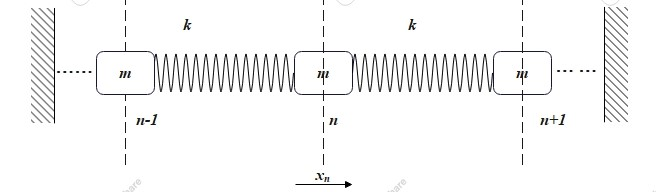
\includegraphics[width=1\textwidth]{Figures/N.jpg}
		\end{framed}
	\caption{ Linear chain of coupled $n$ mass oscillators .}
	\label{fig:N}
\end{figure}

After some time, all the particles of the system oscillate in harmonic oscillating motion with the same angular frequency of $\omega$, but different amplitudes and different
phases. Interestingly, only longitudinal motion (along the chain) in one dimension is considered. We will assume for the time being that all masses $(m)$ and spring constants $(k)$ are equal. Assuming up is the displacement ($x_n$) from equilibrium of mass $n$, then the equation of movements for each mass is given by following equations. 
Consider three adjacent particles with indexes $n - 1$, $n$ and $n + 1$ indicated by in the figure \ref{fig:N}. The equation of motion of the $n^{th}$, $(n-1)^{th}$ and $(n+1)^{th}$  of the particles which is given by,  

\begin{equation}
    m\Ddot{x_{n-1}} = k(2x_{n-1}+x_{n-2} + x_{n} )=0
\end{equation}

\begin{equation}
\label{Jo}
       m\Ddot{x_{n}} = k(x_{n-1}+2x_n - x_{n+1} )=0
\end{equation}

\begin{equation}
       m\Ddot{x_{n+1}} = k(x_{n-1}+ x_n - 2x_{n+1} )=0
\end{equation}

The periodic solutions to the equation of motion, so we might expect the solution to have the form.

\begin{equation}
\label{j1}
    x_{n-1} = Aexp[i(\omega t - k_p(c-1)d)]
\end{equation}

\begin{equation}
\label{j2}
    x_{n} = Aexp[i(\omega t - k_pcd)]
\end{equation}

\begin{equation}
\label{j3}
    x_{n+1} = Aexp[i(\omega t - k_p(c+1)d)]
\end{equation}

$A$ = number of particles in the system \\
$\omega$ = angular frequency \\
$k_p$ = propagation constant \\
$k$ = spring constant

Note that the mass are situated on equally spaced sites with a separation distance $d$. 

\subsection{Dispersion Relation}
\paragraph{}
The acceleration of a specific mass is determined not only by its own displacement, but also by the displacements of its neighbours. And also, the displacement of mass $n$ for a specific normal mode with frequency $\omega$ can be represented as  equation in \eqref{j2}. The coefficients $A$ give the amplitudes of the oscillations for the various masses $n$. Furthermore, substitution of equations \eqref{j1}, \eqref{j2} and \eqref{j3} into equation \eqref{Jo} results in,

\begin{equation}
    -m\omega^2 = k[(exp(ik_p d) + exp(-ik_P d)-2]
\end{equation}

\begin{equation}
    -m\omega^2 = 2k[cos(k_pd)-1]
\end{equation}

\begin{equation}
    \omega = \sqrt{\frac{4k}{m}}sin(\frac{k_pd}{2})
\end{equation}

\begin{equation}
    \omega_0 = \sqrt{\frac{4k}{m}}
\end{equation}

The maximum angular velocity is $\omega_0$. And  phase velocity is $v_p$ and maximum phase velocity we can say $v_{max}$ by substitution \eqref{vp}. 

\begin{equation}
\label{vp}
    v_P = \frac{\omega}{k_p}
\end{equation}

\begin{equation}
    v_{max} = v_0 = d\sqrt{\frac{k}{m}}
\end{equation}

In general, a wave is a superposition of its harmonic components. The envelope or the group of waves are seen to move forward with a velocity $d\omega /  dt$ which is termed the group velocity. 

\begin{equation}
    v_G = \frac{d\omega}{dt}
\end{equation}
\begin{equation}
    V_G = v_0 cos(\frac{k_p d}{2})
\end{equation}

\newpage

\section{Investigate  the two-dimensional spring motion: the mass m is free to move in the $XY$ plane}
\label{XY}
\paragraph{}

It is not insignificant to extend our view of oscillators to other dimensions. In the real world there are many applications that we can see corresponding two-dimensional (2D) systems. Furthermore, this section the two-dimensional spring motion which is about the mass m is free to move in the $xy$ plane will be discussed.

\subsection{Motion for 2D spring motion of a single mass}

\paragraph{}

To obtain the results of 2D spring motion of a single mass we are given a simple task. As early stated in this, the mass m is free to move in the $xy$ plane. It is attached to the solid walls by two unstretched massless springs of spring constant, $k$ aligned along the $x$-axis and by the unstretched massless springs of spring constant $k$ oriented along the $y$-axis. Which means a block (mass $m$) is attached to the sides of a square box by 4 springs. The initial length of each spring is $l$. Place the block (mass $m$) at (0,0). The box is placed horizontally on a frictionless surface (ignore gravity). Let $x(t),y(t)$ the position of the block in time. Considering the given initial conditions and parameters the motion of the mass in the $xy$ plane in the small oscillation approximation will be investigated.

 
\begin{table}[hbt!]
\begin{center}
    \begin{tabular}{|p{8cm}|p{2cm}|}
    \hline
    \textbf{Description of constant} & \textbf{Constant} 
    \\
    \hline
      Spring constant   & $k$ \\
      \hline
     Initial length of each string & $l$ \\
     \hline
     Single mass & $m$ \\
     \hline
     Position of the block in time $x$ direction & $x(t)$ \\
     \hline
     Position of the block in time $y$ direction & $y(t)$ \\
     \hline
    \end{tabular}
    \caption{Description of the constant}
    \label{tab1}
    \end{center}
\end{table}

In the given above table \ref{tab1} explained the meaning of each and each constants that we have been using during our experiment. The place of block (mass $m$) at position (0,0) shown as given below figure \ref{fig:8}. After the change of lengths of the springs when the block is removed from the central position despicts in figure \ref{fig:9}. 

\newpage

\begin{figure}[hbt!]
	\centering
	\begin{framed}
	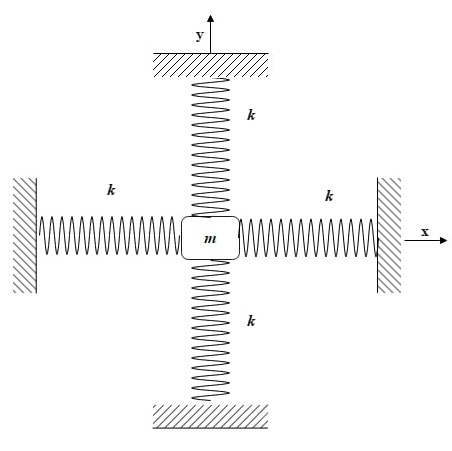
\includegraphics[width=0.5\textwidth]{Figures/H.jpeg}
	\end{framed}
	\caption{ The place of block (mass $m$) at position (0,0).}
	\label{fig:8}
\end{figure}

\begin{figure}[hbt!]
	\centering
	\begin{framed}
	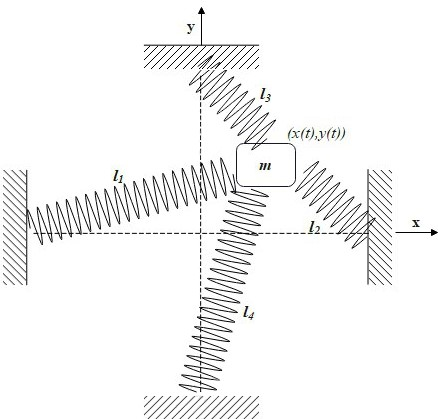
\includegraphics[width=0.53\textwidth]{Figures/I.jpeg}
	\end{framed}
	\caption{ The place of block (mass $m$) at position $(x(t),y(t))$.}
	\label{fig:9}
\end{figure}

\newpage 

Let's consider the stretched length of the given four strings. Those are called as $l_1,l_2,l_3$ and $l_4$ in respectively. 

\begin{equation}
    \label{s1}
    l^2_1 = (x+l)^2+y^2
\end{equation}

\begin{equation}
    \label{s2}
    l^2_2 = (x-l)^2+y^2
\end{equation}

\begin{equation}
    \label{s3}
    l^2_3 = (y+l)^2+x^2
\end{equation}

\begin{equation}
    \label{s4}
    l^2_4 = (y-l)^2+x^2
\end{equation}

Thus, $l_1,l_2,l_3$ and $l_4$ we can write as, 

\begin{equation}
    \label{s11}
    l_1 = \sqrt{(x+l)^2+y^2}
\end{equation}

\begin{equation}
    \label{s22}
    l_2 = \sqrt{(x-l)^2+y^2}
\end{equation}

\begin{equation}
    \label{s33}
    l_3 = \sqrt{(y+l)^2+x^2}
\end{equation}

\begin{equation}
    \label{s44}
    l_4 = \sqrt{(y-l)^2+x^2}
\end{equation}

Since we have stretched length of each springs $l_1,l_2,l_3$ and $l_4$, now we consider the each tension of which all are deforming during the experiment. Each of tension were defined as below. 


\begin{equation}
    \label{t1}
    F_1 = k(\sqrt{(x+l)^2+y^2}- l^2 )^2
\end{equation}

\begin{equation}
    \label{t2}
    F_2 = k(\sqrt{(x-l)^2+y^2}- l^2 )^2
\end{equation}

\begin{equation}
    \label{t3}
    F_3 = k(\sqrt{x^2+(y+l)^2}- l^2 )^2
\end{equation}

\begin{equation}
    \label{t4}
    F_4 = k(\sqrt{x^2+(y-l)^2}- l^2 )^2
\end{equation}

As early discussed, in this project we are not solving given tasks by using Newton's second law \cite{ghayesh2012nonlinear}. Therefore we have to use an alternative option which is called as Euler's lagrange equation. We discussed more details and much needed background about Euler's lagrange in section \ref{lag}. As early stated Euler's lagrange has two major components. Which is known as kinetic energy and potential energy. During the this kind of problems kinetic energy and potential energy play a major role. Therefore, before the solve obtained differential equations it would be prefer to look at governing equations (which may obtained using Euler's lagrange equations ) as much as possible. Because final outputs and their accuracy depend on the initial steps, what we have been used.  

\newpage 

\subsection{Equations of motion for 2D spring motion of a single mass}
\label{xo}

In this section, more details regarding Euler's lagrange equation, governing equations and scientific background about deriving relevant equations will be discussed. As mentioned earlier, before the obtain governing equations we have to be concerned about identifying kinetic energy and potential energy. Therefore, the terms of kinetic energy and potential energy are listed below. Let $V_1,V_2,V_3$ and $V_4$ are potential energies and $T$ is kinetic energy of particle (mass $m$). 

The kinetic energy due to the motion of the mass,

\begin{equation}
\label{k1}
    T = \frac{1}{2}m(\dot{x}^2 + \dot{y}^2)
\end{equation}

The potential energy due to the motion of the mass,

\begin{equation}
    \label{v1}
    V_1 = \frac{1}{2}k(\sqrt{(x+l)^2+y^2}- l^2 )^2
\end{equation}

\begin{equation}
    \label{v2}
    V_2 = \frac{1}{2}k(\sqrt{(x-l)^2+y^2}- l^2 )^2 
\end{equation}

\begin{equation}
    \label{v3}
    V_3 = \frac{1}{2}k(\sqrt{x^2+(y+l)^2}- l^2 )^2 
\end{equation}

\begin{equation}
    \label{v4}
    V_4 =  \frac{1}{2}k(\sqrt{x^2+(y-l)^2}- l^2 )^2
\end{equation}

Let, we can write total potential energy due to the motion of the particle (mass $m$) as shown equation \eqref{V}.

\begin{equation}
    V = V_1+V_2+V_3+V_4
\end{equation}

\begin{align}
\label{V}
\begin{split}
    V = \frac{1}{2}k(\sqrt{x^2+(y-l)^2}- l^2 )^2+ \frac{1}{2}k(\sqrt{(x+l)^2+y^2}- l^2 )^2 +  \frac{1}{2}k(\sqrt{x^2+(y+l)^2}- l^2 )^2    \\ + \frac{1}{2}k(\sqrt{(x-l)^2+y^2}- l^2 )^2 
    \end{split}
\end{align}

Then applying both equations \eqref{k1} and \eqref{V} into the lagrange equation \eqref{3}. 



\begin{align}
\label{L1}
    \begin{split}
        L = \frac{1}{2}m(\dot{x}^2 + \dot{y}^2) - \bigg ( \frac{1}{2}k(\sqrt{x^2+(y-l)^2}- l^2 )^2 + \\ \frac{1}{2}k(\sqrt{(x+l)^2+y^2}- l^2 )^2 + \\ \frac{1}{2}k(\sqrt{x^2+(y+l)^2}- l^2 )^2  + \\\frac{1}{2}k(\sqrt{(x-l)^2+y^2}- l^2 )^2 \bigg )
    \end{split}
\end{align}

In this special case (2D motion for 2D spring motion of a single mass) we have define lagrange equations as below. 

\begin{equation}
    \label{X}
    \frac{d}{dt}(\frac{\partial L}{\partial \dot{x}})-\frac{\partial L}{\partial x}  = 0 
\end{equation}

\begin{equation}
    \label{Y}
     \frac{d}{dt}(\frac{\partial L}{\partial \dot{y}})-\frac{\partial L}{\partial y} = 0
\end{equation}

First, consider both equation \eqref{L1} and equation \eqref{X} simultaneously to obtain motion of particle (mass $m$) direction to $x$.

\begin{align*}
  \frac{d}{dt}(\frac{\partial L}{\partial \dot{x}})-\frac{\partial L}{\partial x}  = 0  
\end{align*}

\begin{align}
\label{X1}
\begin{split}
      m \Dot{x} - \bigg[ \dfrac{kx\left(\sqrt{x^2+\left(y-l\right)^2}-l^2\right)}{\sqrt{x^2+\left(y-l\right)^2}} +   { \dfrac{k\left(x+l\right)\left(\sqrt{\left(x+l\right)^2+y^2}-l^2\right)}{\sqrt{\left(x+l\right)^2+y^2}}
} +  \dfrac{kx\left(\sqrt{x^2+\left(y+l\right)^2}-l^2\right)}{\sqrt{x^2+\left(y+l\right)^2}} \\ + \dfrac{k\left(\sqrt{\left(x-l\right)^2+y^2}-l^2\right)^2}{2}
\bigg]& = 0 
    \end{split}
\end{align}

After that, consider both equation \eqref{L1} and equation \eqref{Y} simultaneously to obtain motion of particle (mass $m$) direction to $y$.

\begin{align*}
   \frac{d}{dt}(\frac{\partial L}{\partial \dot{y}})-\frac{\partial L}{\partial y} = 0
\end{align*}


\begin{align}
\label{Y1}
    \begin{split}
          m \Dot{y} - \bigg[ \dfrac{k\left(y-l\right)\left(\sqrt{\left(y-l\right)^2+x^2}-l^2\right)}{\sqrt{\left(y-l\right)^2+x^2}}  + \dfrac{ky\left(\sqrt{y^2+\left(x+l\right)^2}-l^2\right)}{\sqrt{y^2+\left(x+l\right)^2}} + \dfrac{k\left(y+l\right)\left(\sqrt{\left(y+l\right)^2+x^2}-l^2\right)}{\sqrt{\left(y+l\right)^2+x^2}}\\+ \dfrac{ky\left(\sqrt{y^2+\left(x-l\right)^2}-l^2\right)}{\sqrt{y^2+\left(x-l\right)^2}}
\bigg]& = 0   \\
    \end{split}
\end{align}

\newpage

The tension in the first spring of length $l_1$ is $F_1 \approx k (a+ x – l) = kx$. Magnitude of  $x$-component of this tension is $F_1 cosθ_1 \approx F_1 = kx$ since the angle $\theta_1$ made by $l_1$ with the x-axis is small. Therefore, we find that the x-component of the return force is entirely due to the two springs of lengths $l_1$ and $l_2$. 
\begin{equation}
    F_x = -2kx
\end{equation}

The two springs of lengths $l_3$ and $l_4$ are also totally responsible for the y-component of the return force,

\begin{equation}
     F_y = -2ky
\end{equation}

As a result,  two uncoupled differential equations for the mass m along the x- and y-axes were obtained as below shown.

\begin{equation}
    m\Ddot{x} = -2kx
\end{equation}

\begin{equation}
    m\Ddot{y} = -2ky
\end{equation}

The solutions of these two equations were determined as shown in equations \eqref{so1} and \eqref{so2}.

\begin{equation}
    \label{so1}
    x = A cos(\omega t + \delta_1)
\end{equation}

\begin{equation}
    \label{so2}
    Y = B cos(\omega t + \delta_2)
\end{equation}

In here, $A$, $B$, $\delta_1$, and $\delta_2$ are arbitrary integration constants. We can significantly shorten the previous equations by changing the origin of time. 

\begin{equation}
t\rightarrow t' + \delta_1/\omega
\end{equation}

Hence, we obtain,

\begin{equation}
\label{f1}
    x = A\,\cos(\omega\,t')
\end{equation}

\begin{equation}
\label{f2}
    y = B\,\cos(\omega\,t'-\Delta)
\end{equation}

where ${\mit\Delta}=\phi_2-\phi_1$. 

It is important to note that the motion is obviously periodic in time, with a period of $T=2\pi/ \omega$. As a result, the particle must follow a closed route in the $x$-$y$ plane.













